\section{Group Heat Recovery}\label{group-heat-recovery}

\subsection{HeatExchanger:AirToAir:FlatPlate}\label{heatexchangerairtoairflatplate}

The air-to-air flat plate heat exchanger is an HVAC component typically used for exhaust or relief air heat recovery. The user can choose the flow arrangement type: counter flow, parallel flow, or cross flow with both streams unmixed. The input requires no geometric data. Performance is defined by specifying primary outlet air temperature at nominal (user specified) inlet conditions. In addition, the ratio (h\(^{.}\)A)\(_{p}\) / (h\(^{.}\)A)\(_{s}\) at nominal flow needs to be input, where h is the convective heat transfer coefficient, A is the surface area, p stands for primary side, s for secondary side.

If the heat exchanger is operated in conjunction with an outdoor air economizer (economizer lockout set to \emph{Yes}), the nominal supply air flow rate should be set equal to the minimum outdoor air flow rate specified in the \hyperref[controlleroutdoorair]{Controller:OutdoorAir}. The heat exchanger detects that the economizer is operating by the fact that its inlet air flow rate is greater than its nominal supply air flow rate.

\subsubsection{Inputs}\label{inputs-021}

\paragraph{Field: Name}\label{field-name-020}

A unique user-assigned name for a particular air-to-air flat plate heat exchanger unit. Any reference to this unit by another object will use this name.

\paragraph{Field: Availability Schedule Name}\label{field-availability-schedule-name-008}

The name of the schedule (ref: Schedule) that denotes whether the unit can run during a given time period. A schedule value of 0 indicates that the unit is off for that time period. A schedule value greater than 0 indicates that the unit can operate during the time period. If this field is blank, the schedule has values of 1 for all time periods.

\paragraph{Field: Flow Arrangement Type}\label{field-flow-arrangement-type}

The user specified flow arrangement of the heat exchanger. The possible inputs are \emph{CounterFlow}, \emph{ParallelFlow}, or \emph{CrossFlowBothUnmixed}.

\paragraph{Field: Economizer Lockout}\label{field-economizer-lockout}

This input denotes whether the heat exchanger unit is locked out (bypassed) when the air-side economizer is operating. Both the economizer and high humidity control (Ref. \hyperref[controlleroutdoorair]{Controller:OutdoorAir}) activate the heat exchanger lockout as specified by this input. The input choices are \emph{Yes} (meaning locked out) or \emph{No}. The default input for this field is Yes.

\paragraph{Field: Ratio of Supply to Secondary hA Values}\label{field-ratio-of-supply-to-secondary-ha-values}

The ratio (h\(^{.}\)A)\(_{p}\) / (h\(^{.}\)A)\(_{s}\) at nominal flow. h is the surface convective heat transfer coefficient, A is the heat transfer area, and p and s stand for primary side and secondary side respectively. A typical value for this ratio is 1.0.

\paragraph{Field: Nominal Supply Air Flow Rate}\label{field-nominal-supply-air-flow-rate}

The nominal primary side air flow rate in cubic meters per second. If the unit is operated in conjunction with an outdoor air economizer this should be equal to the minimum outdoor air flow rate. This field is autosizable.

\paragraph{Field: Nominal Supply Air Inlet Temperature}\label{field-nominal-supply-air-inlet-temperature}

The nominal primary side air inlet temperature in Celsius.

\paragraph{Field: Nominal Supply Air Outlet Temperature}\label{field-nominal-supply-air-outlet-temperature}

The nominal primary side air outlet temperature in Celsius.

\paragraph{Field: Nominal Secondary Air Flow Rate}\label{field-nominal-secondary-air-flow-rate}

The nominal secondary side air flow rate in cubic meters per second. This field is autosizable. It is equal to the primary side air flow rate defined above, if autosized.

\paragraph{Field: Nominal Secondary Air Inlet Temperature}\label{field-nominal-secondary-air-inlet-temperature}

The nominal secondary side air inlet temperature in Celsius.

\paragraph{Field: Nominal Electric Power}\label{field-nominal-electric-power}

The electric consumption rate of the unit in watts. Electric power is considered constant whenever the unit operates. This input can be used to model electric power consumption by controls (transformers, relays, etc.) and/or a motor for a rotary heat exchanger. None of this electric power contributes thermal load to the supply or exhaust air streams. The default value for this field is 0.

\paragraph{Field: Supply Air Inlet Node Name}\label{field-supply-air-inlet-node-name-000}

The name of the HVAC system node from which the unit draws its primary inlet air.

\paragraph{Field: Supply Air Outlet Node Name}\label{field-supply-air-outlet-node-name-000}

The name of the HVAC system node to which the unit sends its primary outlet air.

\paragraph{Field: Secondary Air Inlet Node Name}\label{field-secondary-air-inlet-node-name-001}

The name of the HVAC system node from which the unit draws its secondary inlet air.

\paragraph{Field: Secondary Air Outlet Node Name}\label{field-secondary-air-outlet-node-name-000}

The name of the HVAC system node to which the unit sends its secondary outlet air.

An IDF example:

\begin{lstlisting}

HeatExchanger:AirToAir:FlatPlate,
  OA Heat Recovery 1,         !- Name
  FanAndCoilAvailSched,       !- Availability Schedule Name
  CounterFlow,                !- Flow Arrangement Type
  Yes,                        !- Economizer Lockout
  1.0,                        !- Ratio of Supply to Secondary hA Values
  0.4333,                     !- Nominal Supply Air Flow Rate {m3/s}
  5.0,                        !- Nominal Supply Air Inlet Temperature {C}
  15.0,                       !- Nominal Supply Air Outlet Temperature {C}
  0.4333,                     !- Nominal Secondary Air Flow Rate {m3/s}
  20.0,                       !- Nominal Secondary Air Inlet Temperature {C}
  0.0,                        !- Nominal Electric Power {W}
  Desiccant Process Outlet Node,   !- Supply Air Inlet Node Name
  Heat Recovery Outlet Node,   !- Supply Air Outlet Node Name
  Relief Air Outlet Node,   !- Secondary Air Inlet Node Name
  Heat Recovery Secondary Outlet Node;   !- Secondary Air Outlet Node Name
\end{lstlisting}

\subsubsection{Outputs}\label{outputs-014}

\begin{itemize}
\item
  HVAC,Average,Heat Exchanger Sensible Heating Rate {[}W{]}
\item
  HVAC,Sum,Heat Exchanger Sensible Heating Energy {[}J{]}
\item
  HVAC,Average,Heat Exchanger Latent Gain Rate {[}W{]}
\item
  HVAC,Sum,Heat Exchanger Latent Gain Energy {[}J{]}
\item
  HVAC,Average,Heat Exchanger Total Heating Rate {[}W{]}
\item
  HVAC,Sum,Heat Exchanger Total Heating Energy {[}J{]}
\item
  HVAC,Average,Heat Exchanger Sensible Cooling Rate {[}W{]}
\item
  HVAC,Sum,Heat Exchanger Sensible Cooling Energy {[}J{]}
\item
  HVAC,Average,Heat Exchanger Latent Cooling Rate {[}W{]}
\item
  HVAC,Sum,Heat Exchanger Latent Cooling Energy {[}J{]}
\item
  HVAC,Average,Heat Exchanger Total Cooling Rate {[}W{]}
\item
  HVAC,Sum,Heat Exchanger Total Cooling Energy {[}J{]}
\item
  HVAC,Average,Heat Exchanger Electricity Rate {[}W{]}
\item
  HVAC,Sum,Heat Exchanger Electricity Energy {[}J{]}
\end{itemize}

\paragraph{Heat Exchanger Sensible Heating Rate {[}W{]}}\label{heat-exchanger-sensible-heating-rate-w}

This output is the sensible heating rate of the supply air by the heat exchanger in Watts. This rate is determined using the supply air mass flow rate through the heat exchanger unit, the supply air inlet and outlet conditions, and the specific heat of the inlet supply air. A positive value is reported if the supply air is heated by the heat exchanger, else the rate is set to zero.

\paragraph{Heat Exchanger Sensible Heating Energy {[}J{]}}\label{heat-exchanger-sensible-heating-energy-j}

This output is the sensible heating energy added to the supply air by the heat exchanger in Joules over the timestep being reported.

\paragraph{Heat Exchanger Latent Gain Rate {[}W{]}}\label{heat-exchanger-latent-gain-rate-w}

This output is the latent heating rate (humidification) of the supply air by the heat exchanger in Watts. This rate is determined by taking the difference between the Heat Exchanger Total Heating Rate and the Heat Exchanger Sensible Heating Rate. A positive value is reported if the supply air is humidified by the heat exchanger, else the rate is set to zero.

\paragraph{Heat Exchanger Latent Heating Energy {[}J{]}}\label{heat-exchanger-latent-heating-energy-j}

This output is the latent heating energy added to the supply air by the heat exchanger in Joules over the timestep being reported.

\paragraph{Heat Exchanger Total Heating Rate {[}W{]}}\label{heat-exchanger-total-heating-rate-w}

This output is the total heating rate of the supply air by the heat exchanger in Watts. This rate is determined using the supply air mass flow rate through the heat exchanger unit, and the enthalpy of the supply air entering and leaving the unit. A positive value is reported if the enthalpy of the supply air is increased by the heat exchanger, else the rate is set to zero.

\paragraph{Heat Exchanger Total Heating Energy {[}J{]}}\label{heat-exchanger-total-heating-energy-j}

This output is the total heating energy added to the supply air by the heat exchanger in Joules over the timestep being reported.This output is also added to a meter with ResouceType = EnergyTransfer, EndUseKey = HeatRecoveryforHeating, GroupKey = System (ref. Output:Meter objects).

\paragraph{Heat Exchanger Sensible Cooling Rate {[}W{]}}\label{heat-exchanger-sensible-cooling-rate-w}

This output is the sensible cooling rate of the supply air by the heat exchanger in Watts. This rate is determined using the supply air mass flow rate through the heat exchanger unit, the supply air inlet and outlet conditions, and the specific heat of the inlet supply air. A positive value is reported if the supply air is cooled by the heat exchanger, else the rate is set to zero.

\paragraph{Heat Exchanger Sensible Cooling Energy {[}J{]}}\label{heat-exchanger-sensible-cooling-energy-j}

This output is the sensible cooling energy added to the supply air by the heat exchanger in Joules over the timestep being reported.

\paragraph{Heat Exchanger Latent Cooling Rate {[}W{]}}\label{heat-exchanger-latent-cooling-rate-w}

This output is the latent cooling rate (dehumidification) of the supply air by the heat exchanger in Watts. This rate is determined by taking the difference between the Heat Exchanger Total Cooling Rate and the Heat Exchanger Sensible Cooling Rate. A positive value is reported if the supply air is dehumidified by the heat exchanger, else the rate is set to zero.

\paragraph{Heat Exchanger Latent Cooling Energy {[}J{]}}\label{heat-exchanger-latent-cooling-energy-j}

This output is the latent cooling energy added to the supply air by the heat exchanger in Joules over the timestep being reported.

\paragraph{Heat Exchanger Total Cooling Rate {[}W{]}}\label{heat-exchanger-total-cooling-rate-w}

This output is the total cooling rate of the supply air by the heat exchanger in Watts. This rate is determined using the supply air mass flow rate through the heat exchanger unit, and the enthalpy of the supply air entering and leaving the unit. A positive value is reported if the enthalpy of the supply air is decreased by the heat exchanger, else the rate is set to zero.

\paragraph{Heat Exchanger Total Cooling Energy {[}J{]}}\label{heat-exchanger-total-cooling-energy-j}

This output is the total cooling energy added to the supply air by the heat exchanger in Joules over the timestep being reported. This output is also added to a meter with ResouceType = EnergyTransfer, EndUseKey = HeatRecoveryforCooling, GroupKey = System (ref. Output:Meter objects).

\paragraph{Heat Exchanger Electricity Rate {[}W{]}}\label{heat-exchanger-electric-power-w}

This output is the electric consumption rate of the unit in Watts. This rate is applicable whenever the unit operates (i.e., whenever the unit is scheduled to be available and supply and exhaust air flows exist).

\paragraph{Heat Exchanger Electricity Energy {[}J{]}}\label{heat-exchanger-electric-energy-j}

This output is the electric consumption of the unit in Joules for the timestep being reported. This output is also added to a meter with ResourceType = Electricity, EndUseKey = HeatRecovery, GroupKey = System (ref. Output:Meter objects).

\subsection{HeatExchanger:AirToAir:SensibleAndLatent}\label{heatexchangerairtoairsensibleandlatent}

\begin{figure}[htbp]
\centering
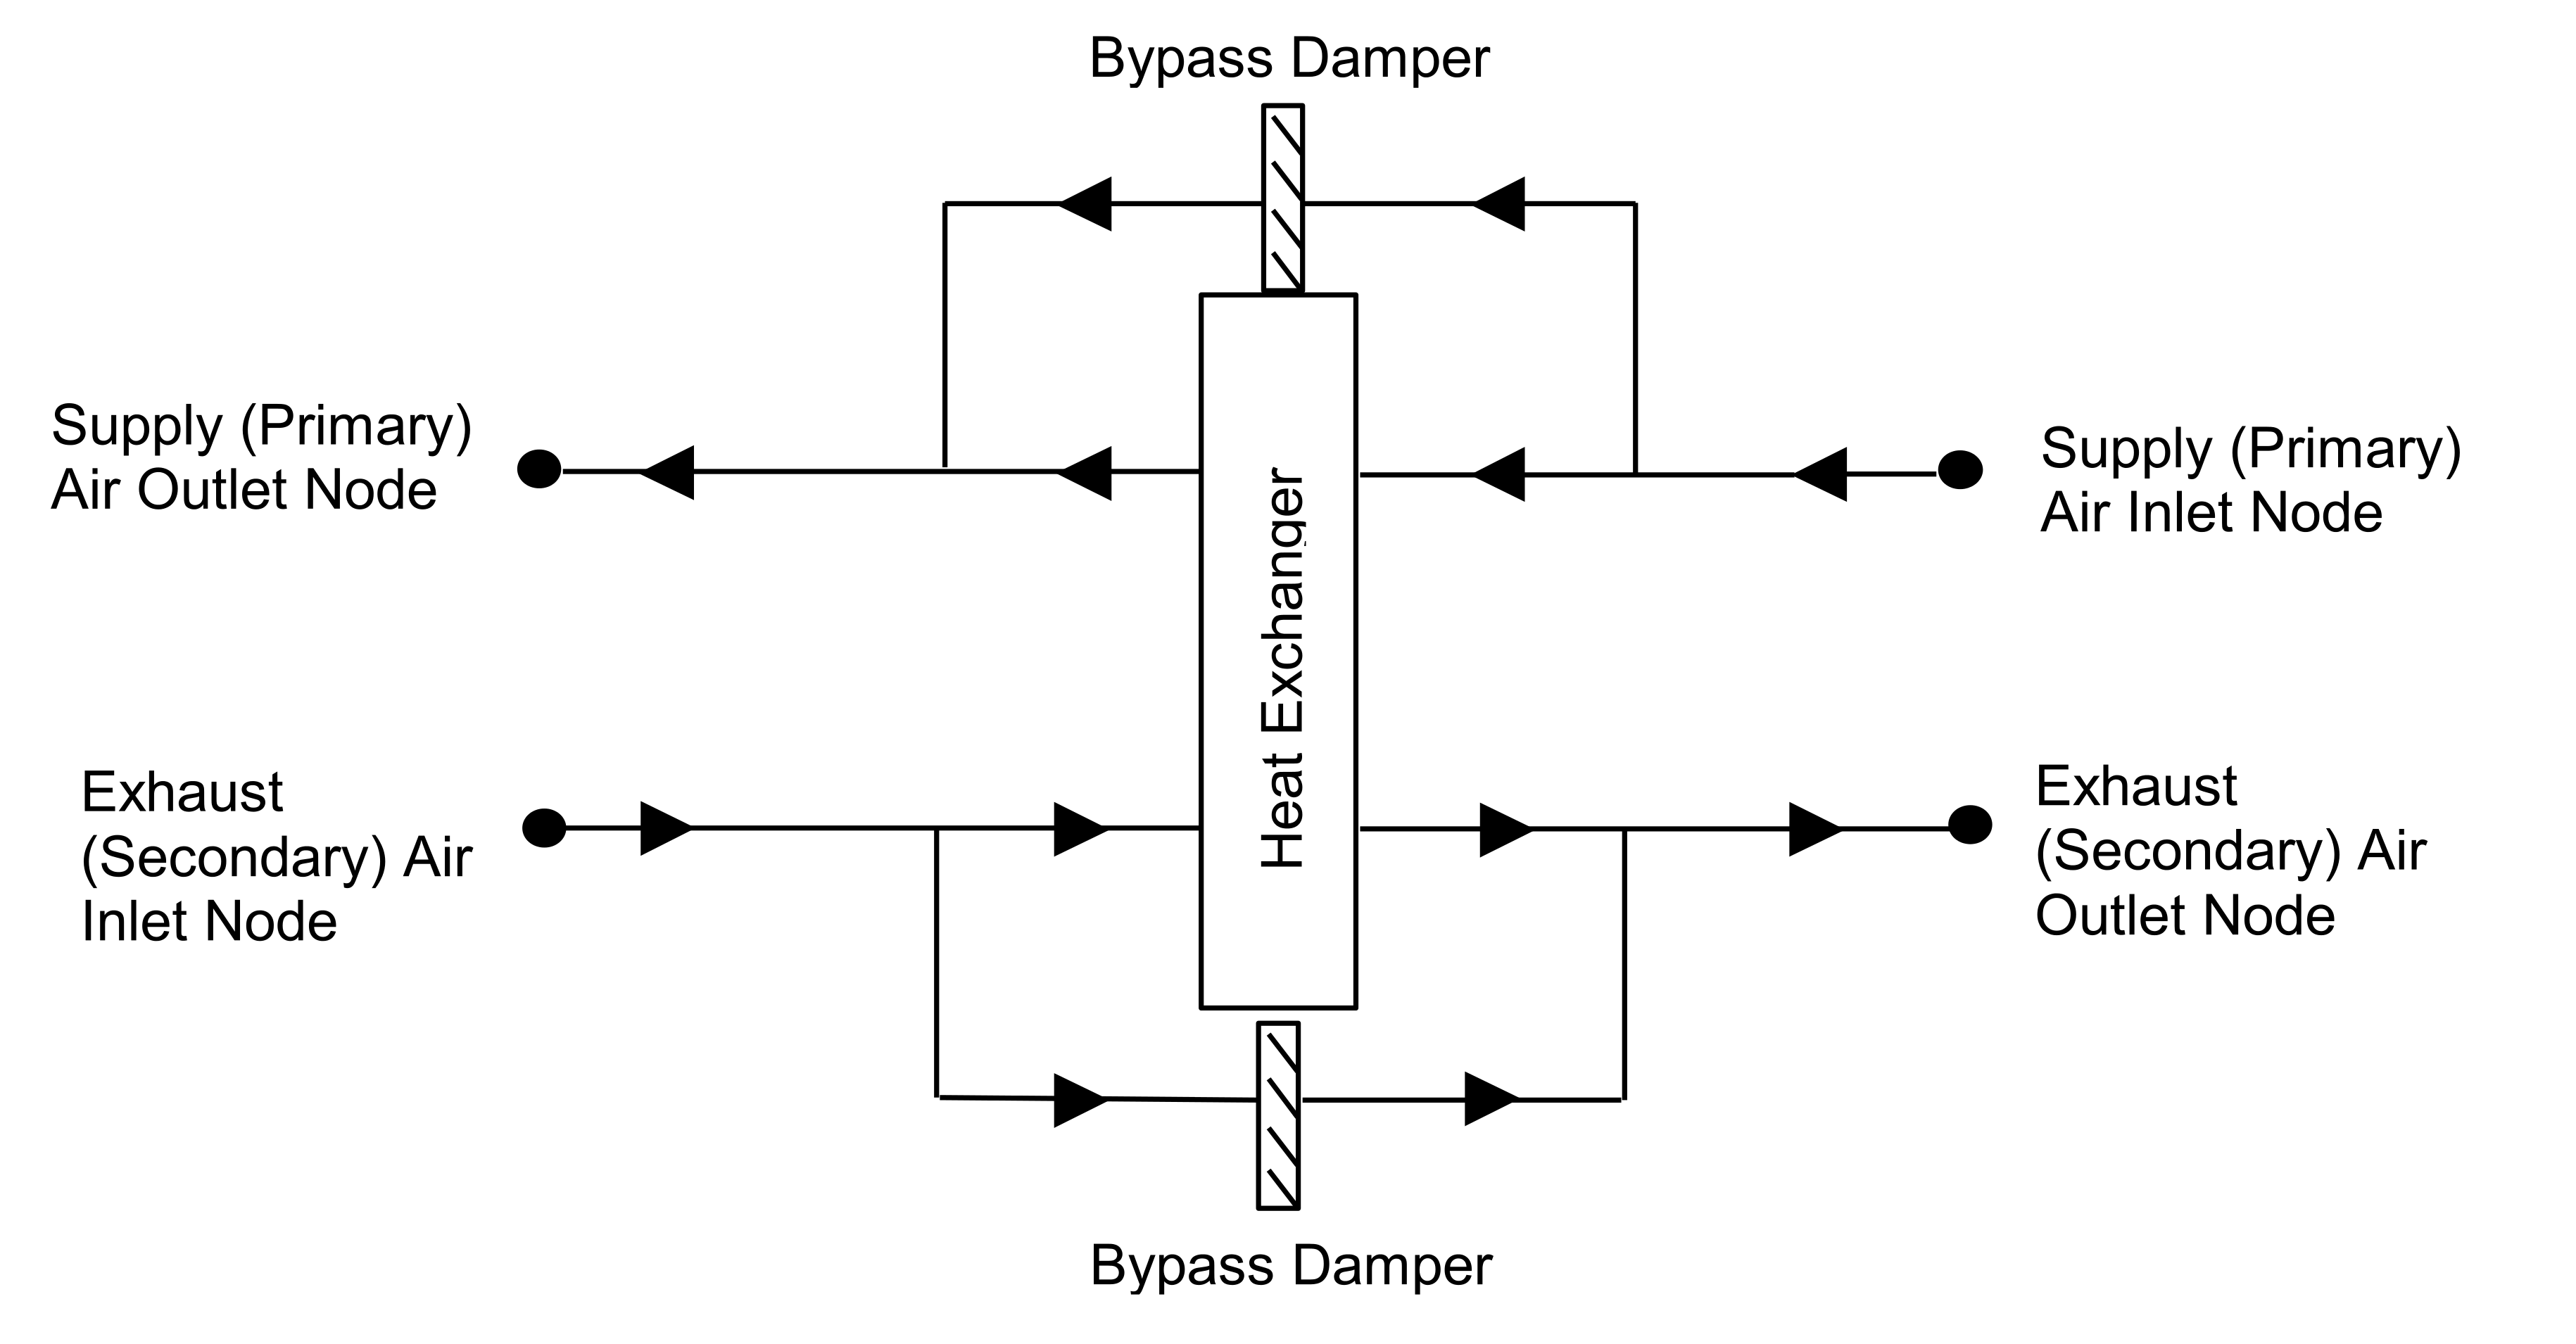
\includegraphics{media/image423.png}
\caption{Schematic of the Sensible and Latent Air-to-Air Heat Exchanger}
\end{figure}

The sensible and latent air-to-air heat exchanger is an HVAC component typically used for exhaust or relief air heat recovery (Figure 150). Heat exchanger performance can be specified to transfer sensible energy, latent energy or both between the supply and exhaust air streams. The input requires no geometric data. Performance is defined by specifying sensible and/or latent effectiveness at 75\% and 100\% of the nominal (rated) supply air flow rate at two operating conditions as shown in Table~\ref{table:operating-conditions-for-defining-heat}.

% table 30
\begin{longtable}[c]{@{}lll@{}}
\caption{Operating Conditions for Defining Heat Exchanger Performance \label{table:operating-conditions-for-defining-heat}} \tabularnewline
\toprule
Parameter & Conditions & \tabularnewline
\midrule
\endfirsthead

\caption[]{Operating Conditions for Defining Heat Exchanger Performance} \tabularnewline
\toprule
Parameter & Conditions & \tabularnewline
\midrule
\endhead

& Heating & Cooling \tabularnewline
Entering supply air temperature: &  &  \tabularnewline
Dry-bulb: & 1.7°C (35°F) & 35°C (95°F) \tabularnewline
Wet-bulb: & 0.6°C (33°F) & 26°C (78°F) \tabularnewline
Entering exhaust air temperature: &  &  \tabularnewline
Dry-bulb: & 21°C (70°F) & 24°C (75°F) \tabularnewline
Wet-bulb: & 14°C (58°F) & 17C (63F) \tabularnewline
\bottomrule
\end{longtable}

Note: Conditions consistent with the Air-Conditioning and Refrigeration Institute's (ARI) Standard 1060-2001.

This object models the basic operation of an air-to-air heat exchanger. Heat exchange between the supply and exhaust air streams occurs whenever the unit is scheduled to be available (Availability schedule) and supply/exhaust air flow is present. This heat exchanger object can be used in conjunction with a conventional air-side economizer (i.e., specify ModulateFlow in the \hyperref[controlleroutdoorair]{Controller:OutdoorAir} object), whereby heat exchange is suspended whenever the air-side economizer (or high humidity control) is active (i.e., air flow is fully bypassed around a fixed-plate heat exchanger or the rotation of a rotary heat exchanger is stopped). This object is also able to suspend heat exchange for the purpose of providing free cooling operation in the absence of a conventional air-side economizer (i.e., specify MinimumFlowWithBypass in the \hyperref[controlleroutdoorair]{Controller:OutdoorAir} object).

During winter weather, humid exhaust air entering the heat exchanger can form frost on the cold heat exchanger surfaces, which can reduce air flow and the amount of energy recovery. Several methods are used to control or eliminate frost formation, and the following types can be modeled for this heat exchanger object: supply air preheat, minimum exhaust air temperature, exhaust air recirculation and exhaust only. For preheat frost control, a separate heating coil object must be placed in the supply inlet air stream to keep the air temperature above the frost threshold temperature. The other frost control types are modeled within this object itself (i.e., do not require a separate object to be defined) based on alpha and numeric inputs to this heat exchanger object.

Air-to-air heat exchangers are sometimes controlled to maintain a fixed supply air outlet temperature to avoid overheating when the heat exchanger is heating the supply (primary) air. To model this control in EnergyPlus, a set point manager object is used to establish a temperature set point at the supply air outlet node of the heat exchanger. Wheel speed modulation or plate supply air bypass is used to control the supply air exiting conditions to this set point. The set point for supply air temperature control should be set at the minimum economizer temperature set point if an air-side economizer is also being used by the air system. If frost control and supply air outlet temperature control are used, frost control takes precedence over supply air temperature control (e.g., frost control defrost time fraction is determined as if wheel speed modulation or plate supply air bypass is not used).

To model a sensible and latent air-to-air heat exchanger located in an air loop, the input data file should include the following objects:

\begin{itemize}
\item
  \hyperref[airloophvacoutdoorairsystem]{AirLoopHVAC:OutdoorAirSystem}
\item
  \hyperref[controlleroutdoorair]{Controller:OutdoorAir}
\item
  \hyperref[outdoorairmixer]{OutdoorAir:Mixer}
\item
  HeatExchanger:AirToAir:SensibleAndLatent
\item
  \hyperref[coilheatingwater]{Coil:Heating:Water}, \hyperref[coilheatingelectric]{Coil:Heating:Electric} or \hyperref[coilheatinggas-000]{Coil:Heating:Fuel} (if preheat frost control is to be modeled)
\item
  \hyperref[setpointmanagerscheduled]{SetpointManager:Scheduled} (if supply air outlet temperature control is used)
\end{itemize}

The sensible and latent air-to-air heat exchanger can also be used in a number of other applications, including conditioning outdoor ventilation air and supplying it directly to a zone without an air loop. See object \hyperref[zonehvacenergyrecoveryventilator]{ZoneHVAC:EnergyRecoveryVentilator} for further details on this specific application.

A description of each input field for this object is provided below.

\subsubsection{Inputs}\label{inputs-1-019}

\paragraph{Field: Name}\label{field-name-1-018}

A unique user-assigned name for a particular sensible/latent air-to-air heat exchanger. Any reference to this heat exchanger by another object will use this name.

\paragraph{Field: Availability Schedule Name}\label{field-availability-schedule-name-1-006}

The name of the schedule (ref: Schedule) that denotes whether the unit can operate during a given time period. A schedule value of less than or equal to 0 indicates that the unit is off for that time period. A schedule value greater than 0 indicates that the unit can operate during the time period. If this field is blank, the schedule has values of 1 for all time periods.

\paragraph{Field: Nominal Supply Air Flow Rate}\label{field-nominal-supply-air-flow-rate-1}

The nominal primary side (supply) air flow rate in cubic meters per second. The actual supply and exhaust air flow rates must be between 50\% and 130\% of this value or a warning will be issued.

\paragraph{Field: Sensible Effectiveness at 100\% Heating Air Flow}\label{field-sensible-effectiveness-at-100-heating-air-flow}

The sensible heat exchange effectiveness at the \emph{heating} condition defined in Table~\ref{table:operating-conditions-for-defining-heat} above with both the supply and exhaust air volume flow rates equal to 100\% of the nominal supply air flow rate specified in the previous input field. The default value for this field is 0.

\paragraph{Field: Latent Effectiveness at 100\% Heating Air Flow}\label{field-latent-effectiveness-at-100-heating-air-flow}

The latent heat exchange effectiveness at the \emph{heating} condition defined in Table~\ref{table:operating-conditions-for-defining-heat} with both the supply and exhaust air volume flow rates equal to 100\% of the nominal supply air flow rate. Specify this value as 0.0 if the heat exchanger does not transfer latent energy. The default value for this field is 0.

\paragraph{Field: Sensible Effectiveness at 75\% Heating Air Flow}\label{field-sensible-effectiveness-at-75-heating-air-flow}

The sensible heat exchange effectiveness at the \emph{heating} condition defined in Table~\ref{table:operating-conditions-for-defining-heat} with both the supply and exhaust air volume flow rates equal to 75\% of the nominal supply air flow rate. The default value for this field is 0.

\paragraph{Field: Latent Effectiveness at 75\% Heating Air Flow}\label{field-latent-effectiveness-at-75-heating-air-flow}

The latent heat exchange effectiveness at the \emph{heating} condition defined in Table~\ref{table:operating-conditions-for-defining-heat} with both the supply and exhaust air volume flow rates equal to 75\% of the nominal supply air flow rate. Specify this value as 0.0 if the heat exchanger does not transfer latent energy. The default value for this field is 0.

\paragraph{Field: Sensible Effectiveness at 100\% Cooling Air Flow}\label{field-sensible-effectiveness-at-100-cooling-air-flow}

The sensible heat exchange effectiveness at the \emph{cooling} condition defined in Table~\ref{table:operating-conditions-for-defining-heat} with both the supply and exhaust air volume flow rates equal to 100\% of the nominal supply air flow rate. The default value for this field is 0.

\paragraph{Field: Latent Effectiveness at 100\% Cooling Air Flow}\label{field-latent-effectiveness-at-100-cooling-air-flow}

The latent heat exchange effectiveness at the \emph{cooling} condition defined in Table~\ref{table:operating-conditions-for-defining-heat} with both the supply and exhaust air volume flow rates equal to 100\% of the nominal supply air flow rate. Specify this value as 0.0 if the heat exchanger does not transfer latent energy. The default value for this field is 0.

\paragraph{Field: Sensible Effectiveness at 75\% Cooling Air Flow}\label{field-sensible-effectiveness-at-75-cooling-air-flow}

The sensible heat exchange effectiveness at the \emph{cooling} condition defined in Table~\ref{table:operating-conditions-for-defining-heat} with both the supply and exhaust air volume flow rates equal to 75\% of the nominal supply air flow rate. The default value for this field is 0.

\paragraph{Field: Latent Effectiveness at 75\% Cooling Air Flow}\label{field-latent-effectiveness-at-75-cooling-air-flow}

The latent heat exchange effectiveness at the \emph{cooling} condition defined in Table~\ref{table:operating-conditions-for-defining-heat} with both the supply and exhaust air volume flow rates equal to 75\% of the nominal supply air flow rate. Specify this value as 0.0 if the heat exchanger does not transfer latent energy. The default value for this field is 0.

\paragraph{Field: Supply Air Inlet Node Name}\label{field-supply-air-inlet-node-name-1-000}

The name of the HVAC system node from which the unit draws its supply (primary) inlet air.

\paragraph{Field: Supply Air Outlet Node Name}\label{field-supply-air-outlet-node-name-1}

The name of the HVAC system node to which the unit sends its supply (primary) outlet air.

\paragraph{Field: Exhaust Air Inlet Node Name}\label{field-exhaust-air-inlet-node-name}

The name of the HVAC system node from which the unit draws its exhaust (secondary) inlet air.

\paragraph{Field: Exhaust Air Outlet Node Name}\label{field-exhaust-air-outlet-node-name}

The name of the HVAC system node to which the unit sends its exhaust (secondary) outlet air.

\paragraph{Field: Nominal Electric Power}\label{field-nominal-electric-power-1}

The electric consumption rate of the unit in watts. Electric power is considered constant whenever the unit operates. This numeric input can be used to model electric power consumption by controls (transformers, relays, etc.) and/or a motor for a rotary heat exchanger. None of this electric power contributes thermal load to the supply or exhaust air streams. The default value for this field is 0.

\paragraph{Field: Supply Air Outlet Temperature Control}\label{field-supply-air-outlet-temperature-control}

This alpha field determines if the heat exchanger's supply air outlet is controlled to a temperature set point when the heat exchanger is actively conditioning the supply (primary) air. The choices for this input field are Yes or No, with the default being No. When supply air outlet temperature control is used, the wheel rotational speed modulates or supply air is bypassed around the plate heat exchanger to maintain the desired setpoint temperature. A setpoint manager object is required to establish the desired set point at the supply air outlet node (reference: \hyperref[setpointmanagerscheduled]{SetpointManager:Scheduled}). When an air-side economizer is also being modeled for this air system, the heat exchanger is deactivated during economizer operation. Additionally, the set point for the supply air outlet temperature control should be equal to the economizer outdoor air temperature lower limit (reference: \hyperref[controlleroutdoorair]{Controller:OutdoorAir}, field Economizer Minimum Limit Dry-Bulb Temperature), however, any temperature set point may be used.

\paragraph{Field: Heat Exchanger Type}\label{field-heat-exchanger-type}

This alpha field denotes the type of heat exchanger being modeled: Plate (e.g., fixed plate) or Rotary (e.g., rotating cylinder or wheel). The default choice for this field is Plate . The heat exchanger type affects the modeling of frost control options and supply air outlet temperature control. For rotary heat exchangers, rotational speed is varied to control frost formation or the supply air outlet temperature. For plate exchangers, air bypass around the heat exchanger is used to obtain the desired effect.

\paragraph{Field: Frost Control Type}\label{field-frost-control-type}

This alpha field has four choices: None, ExhaustAirRecirculation, ExhaustOnly and MinimumExhaustTemperature. If this field is left blank, the default frost control type is None . For modeling preheat frost control, specify None for this input field and insert a separate heating coil object in the supply inlet air stream to keep the air temperature above the desired frost threshold temperature.

\emph{ExhaustAirRecirculation}: dampers are used to direct exhaust air back into the zone through the supply side of the heat exchanger when the supply (outdoor) air inlet temperature falls below a threshold temperature (defined in the next input field). The fraction of time that exhaust air is circulated through the supply side of the heat exchanger is dependent on the supply (outdoor) air inlet temperature with respect to the threshold temperature, the initial defrost time fraction, and the rate of change of defrost time fraction (see \emph{Field: Rate of Defrost Time Fraction Increase}). When exhaust air is being recirculated, no supply (outdoor ventilation) air is being provided through the heat exchanger unit (which may or may not be acceptable regarding ventilation for occupants).

\emph{ExhaustOnly (supply air bypass)}: this control cycles off the supply air flow through the heat exchanger for a certain period of time while the exhaust air continues to flow through the exhaust side of the heat exchanger. The fraction of time that the supply flow through the heat exchanger is cycled off is dependent on the supply (outdoor) air inlet temperature with respect to the threshold temperature, the initial defrost time fraction, and the rate of change of defrost time fraction (see \emph{Field: Rate of Defrost Time Fraction Increase}). When implemented in real applications, provisions are usually made to avoid building depressurization when this frost control is operating (automatic or pressure-operated dampers, or a bypass air damper around the supply side of the heat exchanger). For this frost control type, it is assumed that the supply air is bypassed around the heat exchanger during frost control operation (i.e., the total supply flow is not reduced during defrost, but merely bypassed around the heat exchanger).

\emph{MinimumExhaustTemperature}: the temperature of the exhaust air leaving the heat exchanger is monitored and the heat exchanger effectiveness is decreased (by slowing heat exchanger rotation or bypassing supply air around the plate exchanger) to keep the exhaust air from falling below the threshold temperature.

\paragraph{Field: Threshold Temperature}\label{field-threshold-temperature}

This numeric field defines the dry-bulb temperature of air which is used to initiate frost control. The default value is 1.7 °C. For ExhaustAirRecirculation and ExhaustOnly frost control, the threshold temperature defines the supply (outdoor) air inlet temperature below which frost control is active. For MinimumExhaustTemperature frost control, heat exchanger effectiveness is controlled to keep the exhaust air outlet temperature from falling below this threshold temperature value.

The appropriate threshold temperature varies with exhaust (inlet) air temperature and humidity, frost control type, heat exchanger type, and whether the heat exchanger transfers sensible energy alone or both sensible and latent energy (enthalpy). Typical threshold temperatures are provided in Table~\ref{table:typical-threshold-temperatures} below. However, it is recommended that the user consult manufacturer's information for the specific air-to-air heat exchanger being modeled.

% table 31
\begin{longtable}[c]{>{\raggedright}p{1.5in}>{\raggedright}p{1.5in}>{\raggedright}p{1.5in}>{\raggedright}p{1.5in}}
\caption{Typical threshold temperatures \label{table:typical-threshold-temperatures}} \tabularnewline
\toprule
Frost Control Type & Heat Exchanger Type & Energy Exchange & Threshold Temperature \tabularnewline
\midrule
\endfirsthead

\caption[]{Typical threshold temperatures} \tabularnewline
\toprule
Frost Control Type & Heat Exchanger Type & Energy Exchange & Threshold Temperature \tabularnewline
\midrule
\endhead

Exhaust Air Recirculation & Plate & Sensible-only & -1.1°C (30°F) \tabularnewline
Exhaust Air Recirculation & Plate & Sensible + latent & -12.2°C (10°F) \tabularnewline
Exhaust Air Recirculation & Rotary & Sensible-only & -12.2°C (10°F) \tabularnewline
Exhaust Air Recirculation & Rotary & Sensible + latent & -23.3°C (-10°F) \tabularnewline

Exhaust only & Plate & Sensible-only & -1.1°C (30°F) \tabularnewline
Exhaust only & Plate & Sensible + latent & -12.2°C (10°F) \tabularnewline
Exhaust only & Rotary & Sensible-only & -12.2°C (10°F) \tabularnewline
Exhaust only & Rotary & Sensible + latent & -23.3°C (-10°F) \tabularnewline

Minimum exhaust temperature & Plate & Sensible-only & 1.7°C (35°F) \tabularnewline
Minimum exhaust temperature & Plate & Sensible + latent & 1.7°C (35°F) \tabularnewline
Minimum exhaust temperature & Rotary & Sensible-only & 1.7°C (35°F) \tabularnewline
Minimum exhaust temperature & Rotary & Sensible + latent & 1.7°C (35°F) \tabularnewline

Preheat** & Plate & Sensible-only & -1.1°C (30°F) \tabularnewline
Preheat** & Plate & Sensible + latent & -12.2°C (10°F) \tabularnewline
Preheat** & Rotary & Sensible-only & -12.2°C (10°F) \tabularnewline
Preheat** & Rotary & Sensible + latent & -23.3°C (-10°F) \tabularnewline
\bottomrule
\end{longtable}

Source: Indoor Humidity Assessment Tool, U.S. Environmental Protection Agency,\url{http://www.epa.gov/iaq/schooldesign/saves.html}

** To model preheat frost control, specify frost control type as None and place a heating coil in the supply inlet air stream controlled to the keep the air temperature above the frost threshold temperature.

\paragraph{Field: Initial Defrost Time Fraction}\label{field-initial-defrost-time-fraction}

This numeric field defines the fraction of the simulation timestep when frost control will be invoked when the threshold temperature is reached. This field is only used for the ExhaustAirRecirculation and ExhaustOnly frost control types. The value for this field must be ≥ 0 and ≤ 1. The default time fraction is 0.083 (e.g., 5 min / 60 min) which is typical for ExhaustAirRecirculation frost control. Higher initial defrost time fractions (e.g., 0.167 = 10 min / 60 min) are typically required for ExhaustOnly frost control. For best results, the user should obtain this information from the manufacturer.

\paragraph{Field: Rate of Defrost Time Fraction Increase}\label{field-rate-of-defrost-time-fraction-increase}

This numeric field defines the rate of increase in the defrost time fraction as the supply (outdoor) air inlet temperature falls below the threshold temperature. This field is only used for the ExhaustAirRecirculation and ExhaustOnly frost control types. The value for this field must be ≥ 0. The default value is 0.012 (e.g., 0.72 min / 60 min per degree C temperature difference) which is typical for ExhaustAirRecirculation frost control. Higher values (e.g., 0.024 = 1.44 min / 60 min per degree C temperature difference) are typically required for ExhaustOnly frost control. For best results, the user should obtain this information from the manufacturer.

This value is used to determine the total defrost time fraction as follows:


Total defrost time fraction = Initial Defrost Time Fraction +
Rate of Defrost Time Fraction Increase * (\(T_{threshold}\) - \(T_{supply air inlet}\))

The model does not allow the total defrost time fraction to exceed 1.0 or be less than 0.

\paragraph{Field: Economizer Lockout}\label{field-economizer-lockout-1}

This input denotes whether the heat exchanger unit is locked out (bypassed for plate type heat exchangers or the rotation is suspended for rotary type heat exchangers) when the air-side economizer is operating. Both the economizer and high humidity control (Ref. \hyperref[controlleroutdoorair]{Controller:OutdoorAir}) activate the heat exchanger lockout as specified by this input. The input choices are \emph{Yes} (meaning locked out) or \emph{No}. The default input for this field is Yes.

Following is an example input for this heat exchanger object:

\begin{lstlisting}

HeatExchanger:AirToAir:SensibleAndLatent,
  OA Heat Recovery 1,         !- Name
  FanAndCoilAvailSched,       !- Availability Schedule Name
  0.4333,                     !- Nominal Supply Air Flow Rate {m3/s}
  .76,                        !- Sensible Effectiveness at 100% Heating Air Flow {dimensionless}
  .68,                        !- Latent Effectiveness at 100% Heating Air Flow {dimensionless}
  .81,                        !- Sensible Effectiveness at 75% Heating Air Flow {dimensionless}
  .73,                        !- Latent Effectiveness at 75% Heating Air Flow {dimensionless}
  .76,                        !- Sensible Effectiveness at 100% Cooling Air Flow {dimensionless}
  .68,                        !- Latent Effectiveness at 100% Cooling Air Flow {dimensionless}
  .81,                        !- Sensible Effectiveness at 75% Cooling Air Flow {dimensionless}
  .73,                        !- Latent Effectiveness at 75% Cooling Air Flow {dimensionless}
  Outside Air Inlet Node Preheated,   !- Supply Air Inlet Node Name
  Heat Recovery Outlet Node,  !- Supply Air Outlet Node Name
  Relief Air Outlet Node,     !- Exhaust Air Inlet Node Name
  Heat Recovery Secondary Outlet Node,   !- Exhaust Air Outlet Node Name
  200.0,                      !- Nominal Electric Power {W}
  No,                         !- Supply Air Outlet Temperature Control
  Plate,                      !- Heat Exchanger Type
  None;                       !- Frost Control Type
\end{lstlisting}

\subsubsection{Outputs}\label{outputs-1-012}

\begin{itemize}
\item
  HVAC,Average,Heat Exchanger Sensible Heating Rate {[}W{]}
\item
  HVAC,Sum,Heat Exchanger Sensible Heating Energy {[}J{]}
\item
  HVAC,Average,Heat Exchanger Latent Gain Rate {[}W{]}
\item
  HVAC,Sum,Heat Exchanger Latent Gain Energy {[}J{]}
\item
  HVAC,Average,Heat Exchanger Total Heating Rate {[}W{]}
\item
  HVAC,Sum,Heat Exchanger Total Heating Energy {[}J{]}
\item
  HVAC,Average,Heat Exchanger Sensible Cooling Rate {[}W{]}
\item
  HVAC,Sum,Heat Exchanger Sensible Cooling Energy {[}J{]}
\item
  HVAC,Average,Heat Exchanger Latent Cooling Rate {[}W{]}
\item
  HVAC,Sum,Heat Exchanger Latent Cooling Energy {[}J{]}
\item
  HVAC,Average,Heat Exchanger Total Cooling Rate {[}W{]}
\item
  HVAC,Sum,Heat Exchanger Total Cooling Energy {[}J{]}
\item
  HVAC,Average,Heat Exchanger Electricity Rate {[}W{]}
\item
  HVAC,Sum,Heat Exchanger Electricity Energy {[}J{]}
\item
  HVAC,Average,Heat Exchanger Sensible Effectiveness{[]}
\item
  HVAC,Average,Heat Exchanger Latent Effectiveness{[]}
\item
  HVAC,Average,Heat Exchanger Supply Air Bypass Mass Flow Rate {[}kg/s{]}
\item
  HVAC,Average,Heat Exchanger Exhaust Air Bypass Mass Flow Rate {[}kg/s{]} HVAC,Average,Heat Exchanger Defrost Time Fraction{[]}
\end{itemize}

\paragraph{Heat Exchanger Sensible Heating Rate {[}W{]}}\label{heat-exchanger-sensible-heating-rate-w-1}

This output is the sensible heating rate of the supply air by the heat exchanger in Watts. This rate is determined using the supply air mass flow rate through the heat exchanger unit, the supply air inlet and outlet conditions, and the specific heat of the inlet supply air. A positive value is reported if the supply air is heated by the heat exchanger, else the rate is set to zero.

\paragraph{Heat Exchanger Sensible Heating Energy {[}J{]}}\label{heat-exchanger-sensible-heating-energy-j-1}

This output is the sensible heating energy added to the supply air by the heat exchanger in Joules over the timestep being reported.

\paragraph{Heat Exchanger Latent Gain Rate {[}W{]}}\label{heat-exchanger-latent-gain-rate-w-1}

This output is the latent heating rate (humidification) of the supply air by the heat exchanger in Watts. This rate is determined by taking the difference between the Heat Exchanger Total Heating Rate and the Heat Exchanger Sensible Heating Rate. A positive value is reported if the supply air is humidified by the heat exchanger, else the rate is set to zero.

\paragraph{Heat Exchanger Latent Gain Energy {[}J{]}}\label{heat-exchanger-latent-gain-energy-j}

This output is the latent heating energy added to the supply air by the heat exchanger in Joules over the timestep being reported.

\paragraph{Heat Exchanger Total Heating Rate {[}W{]}}\label{heat-exchanger-total-heating-rate-w-1}

This output is the total heating rate of the supply air by the heat exchanger in Watts. This rate is determined using the supply air mass flow rate through the heat exchanger unit, and the enthalpy of the supply air entering and leaving the unit. A positive value is reported if the enthalpy of the supply air is increased by the heat exchanger, else the rate is set to zero.

\paragraph{Heat Exchanger Total Heating Energy {[}J{]}}\label{heat-exchanger-total-heating-energy-j-1}

This output is the total heating energy added to the supply air by the heat exchanger in Joules over the timestep being reported.This output is also added to a meter with ResouceType = EnergyTransfer, EndUseKey = HeatRecoveryforHeating, GroupKey = System (ref. Output:Meter objects).

\paragraph{Heat Exchanger Sensible Cooling Rate {[}W{]}}\label{heat-exchanger-sensible-cooling-rate-w-1}

This output is the sensible cooling rate of the supply air by the heat exchanger in Watts. This rate is determined using the supply air mass flow rate through the heat exchanger unit, the supply air inlet and outlet conditions, and the specific heat of the inlet supply air. A positive value is reported if the supply air is cooled by the heat exchanger, else the rate is set to zero.

\paragraph{Heat Exchanger Sensible Cooling Energy {[}J{]}}\label{heat-exchanger-sensible-cooling-energy-j-1}

This output is the sensible cooling energy added to the supply air by the heat exchanger in Joules over the timestep being reported.

\paragraph{Heat Exchanger Latent Cooling Rate {[}W{]}}\label{heat-exchanger-latent-cooling-rate-w-1}

This output is the latent cooling rate (dehumidification) of the supply air by the heat exchanger in Watts. This rate is determined by taking the difference between the Heat Exchanger Total Cooling Rate and the Heat Exchanger Sensible Cooling Rate. A positive value is reported if the supply air is dehumidified by the heat exchanger, else the rate is set to zero.

\paragraph{Heat Exchanger Latent Cooling Energy {[}J{]}}\label{heat-exchanger-latent-cooling-energy-j-1}

This output is the latent cooling energy added to the supply air by the heat exchanger in Joules over the timestep being reported.

\paragraph{Heat Exchanger Total Cooling Rate {[}W{]}}\label{heat-exchanger-total-cooling-rate-w-1}

This output is the total cooling rate of the supply air by the heat exchanger in Watts. This rate is determined using the supply air mass flow rate through the heat exchanger unit, and the enthalpy of the supply air entering and leaving the unit. A positive value is reported if the enthalpy of the supply air is decreased by the heat exchanger, else the rate is set to zero.

\paragraph{Heat Exchanger Total Cooling Energy {[}J{]}}\label{heat-exchanger-total-cooling-energy-j-1}

This output is the total cooling energy added to the supply air by the heat exchanger in Joules over the timestep being reported. This output is also added to a meter with ResouceType = EnergyTransfer, EndUseKey = HeatRecoveryforCooling, GroupKey = System (ref. Output:Meter objects).

\paragraph{Heat Exchanger Electricity Rate {[}W{]}}\label{heat-exchanger-electric-power-w-1}

This output is the electric consumption rate of the unit in Watts. This rate is applicable whenever the unit operates (i.e., whenever the unit is scheduled to be available and supply and exhaust air flows exist).

\paragraph{Heat Exchanger Electricity Energy {[}J{]}}\label{heat-exchanger-electric-energy-j-1}

This output is the electric consumption of the unit in Joules for the timestep being reported. This output is also added to a meter with ResourceType = Electricity, EndUseKey = HeatRecovery, GroupKey = System (ref. Output:Meter objects).

\paragraph{Heat Exchanger Sensible Effectiveness {[]}}\label{heat-exchanger-sensible-effectiveness}

This output is the average sensible effectiveness of the heat exchanger (excluding bypass air, if any) over the timestep being reported.

\paragraph{Heat Exchanger Latent Effectiveness {[]}}\label{heat-exchanger-latent-effectiveness}

This output is the average latent effectiveness of the heat exchanger (excluding bypass air, if any) over the timestep being reported.

\paragraph{Heat Exchanger Supply Air Bypass Mass Flow Rate {[}kg/s{]}}\label{heat-exchanger-supply-air-bypass-mass-flow-rate-kgs}

This output is the average mass flow rate in kg/second of the supply (primary) air stream that is bypassing the heat exchanger over the timestep being reported. This flow rate is equal to the total supply mass flow rate through the heat exchanger \textbf{unit} minus the amount passing through the supply side of the heat exchanger \textbf{core}.

\paragraph{Heat Exchanger Exhaust Air Bypass Mass Flow Rate {[}kg/s{]}}\label{heat-exchanger-exhaust-air-bypass-mass-flow-rate-kgs}

This output is the average mass flow rate in kg/second of the exhaust (secondary) air stream that is bypassing the heat exchanger over the timestep being reported. This flow rate is equal to the total exhaust mass flow rate through the heat exchanger \textbf{unit} minus the amount passing through the exhaust side of the heat exchanger \textbf{core}.

\paragraph{Heat Exchanger Defrost Time Fraction {[]}}\label{heat-exchanger-defrost-time-fraction}

This output is the average fraction of the reporting timestep when frost control is being implemented.

\subsection{HeatExchanger:Desiccant:BalancedFlow}\label{heatexchangerdesiccantbalancedflow}

This desiccant heat exchanger object is an HVAC component used to model both temperature (sensible) and moisture (latent) heat exchange between two air streams (Figure~\ref{fig:schematic-of-the-balanced-flow-desiccant-heat}). The model assumes balanced air flow through the regeneration and process sides of the heat exchanger (i.e., regeneration and process air volume flow rates and face velocities are the same). Heat exchanger performance is specified through a performance data type object (e.g., \hyperref[heatexchangerdesiccantbalancedflowperformancedatatype1]{HeatExchanger:Desiccant:BalancedFlow:PerformanceDataType1}).

\begin{figure}[hbtp] % fig 151
\centering
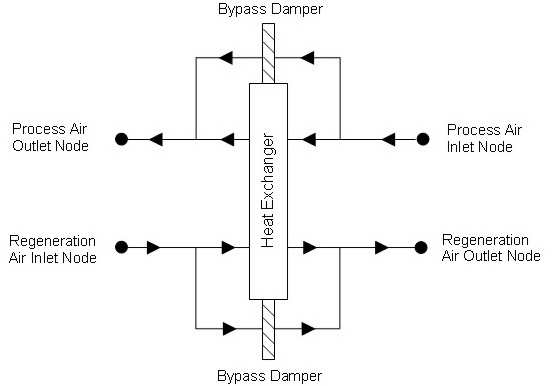
\includegraphics[width=0.9\textwidth, height=0.9\textheight, keepaspectratio=true]{media/image424.png}
\caption{Schematic of the Balanced Flow Desiccant Heat Exchanger \protect \label{fig:schematic-of-the-balanced-flow-desiccant-heat}}
\end{figure}

Currently, this desiccant heat exchanger model can be referenced by two compound objects: \hyperref[coilsystemcoolingdxheatexchangerassisted]{CoilSystem:Cooling:DX:HeatExchangerAssisted} and \hyperref[dehumidifierdesiccantsystem]{Dehumidifier:Desiccant:System}, both of which are used to provide enhanced dehumidification over conventional systems. If this heat exchanger is referenced by a compound object, the compound object will control heat exchanger operation (i.e., tell the heat exchanger if heat exchange is needed or not for each simulation timestep).

This desiccant heat exchanger object may also be specified directly in an \hyperref[airloophvac]{AirLoopHVAC} (air loop \hyperref[branchlist]{BranchList}) or in an \hyperref[airloophvacoutdoorairsystem]{AirLoopHVAC:OutdoorAirSystem} (\hyperref[airloophvacoutdoorairsystemequipmentlist]{AirLoopHVAC:OutdoorAirSystem:EquipmentList}) without being referenced by a compound object. If specified directly in an \hyperref[airloophvac]{AirLoopHVAC} or \hyperref[airloophvacoutdoorairsystem]{AirLoopHVAC:OutdoorAirSystem}, then the heat exchanger can be controlled to provide heat exchange based on a maximum and/or minimum humidity set point placed on the process air outlet node (ref. Setpoint Managers). If no humidity set points are provided on this node, then heat exchange will be provided whenever the heat exchanger is available to operate (via its availability schedule) and there is a temperature and/or humidity ratio difference between the two air streams.

Inputs to this model include an availability schedule name, inlet and outlet air node names, and the type and name of the heat exchanger performance data object. A description of each input field for this object is provided below.

\subsubsection{Inputs}\label{inputs-2-018}

\paragraph{Field: Name}\label{field-name-2-017}

A unique, user-assigned name for a particular balanced flow desiccant heat exchanger. Any reference to this heat exchanger by another object will use this name.

\paragraph{Field: Availability Schedule Name}\label{field-availability-schedule-name-2-003}

The name of the schedule (ref: Schedule) that denotes whether the heat exchanger can operate during a given time period. A schedule value of less than or equal to 0 indicates that the unit is off for that time period. A schedule value greater than 0 indicates that the unit can operate during the time period. If this field is blank, the schedule has values of 1 for all time periods.

\paragraph{Field: Regeneration Air Inlet Node Name}\label{field-regeneration-air-inlet-node-name-000}

The name of the HVAC system node from which the unit draws its regeneration inlet air.

\paragraph{Field: Regeneration Air Outlet Node Name}\label{field-regeneration-air-outlet-node-name}

The name of the HVAC system node to which the unit sends its regeneration outlet air.

\paragraph{Field: Process Air Inlet Node Name}\label{field-process-air-inlet-node-name-000}

The name of the HVAC system node from which the unit draws its process inlet air.

\paragraph{Field: Process Air Outlet Node Name}\label{field-process-air-outlet-node-name-000}

The name of the HVAC system node to which the unit sends its process outlet air.

\paragraph{Field: Heat Exchanger Performance Object Type}\label{field-heat-exchanger-performance-object-type}

This alpha field contains the type of model used to simulate the desiccant heat exchanger's thermal performance and electrical energy use. Currently, the only valid choice is \hyperref[heatexchangerdesiccantbalancedflowperformancedatatype1]{HeatExchanger:Desiccant:BalancedFlow:PerformanceDataType1}.

\paragraph{Field: Heat Exchanger Performance Name}\label{field-heat-exchanger-performance-name}

This alpha field contains the identifying name of the specific heat exchanger performance type object (e.g., \hyperref[heatexchangerdesiccantbalancedflowperformancedatatype1]{HeatExchanger:Desiccant:BalancedFlow:PerformanceDataType1}) that defines the performance for this heat exchanger. A single heat exchanger performance type object may be used to define performance for many HeatExchanger:Desiccant:BalancedFlow objects (i.e., the same name may be used in this input field for more than one balanced flow desiccant heat exchanger).

\paragraph{Field: Economizer Lockout}\label{field-economizer-lockout-2}

This input denotes whether the heat exchanger unit is locked out (heat exchanger rotation is suspended) when the air-side economizer is operating. Both the economizer and high humidity control (Ref. \hyperref[controlleroutdoorair]{Controller:OutdoorAir}) activate the heat exchanger lockout as specified by this input. The input choices are \emph{Yes} (meaning locked out) or \emph{No}. Economizer lockout is typically \emph{not} used for this type of heat exchanger. For this reason, the default input for this field is No.

Following is an example input for this heat exchanger object:

\begin{lstlisting}

HeatExchanger:Desiccant:BalancedFlow,
  Desiccant Heat Exchanger 1,                 !- Name
  OfficeHeatCoolAvail,                               !- Availability Schedule Name
  DXSystem 1 Mixed Air Node,                   !- Regeneration Air Inlet Node Name
  DX Cooling Coil Air Inlet Node,         !- Regeneration Air Outlet Node Name
  DX Cooling Coil Air Outlet Node,       !- Process Air Inlet Node Name
  DXSystem 1 Fan Air Inlet Node,           !- Process Air Outlet Node Name
  HeatExchanger:Desiccant:BalancedFlow:PerformanceDataType1, !- Heat Exchanger Performance Object Type
  HXDesPerf1;                                                 !- Heat Exchanger Performance Name
\end{lstlisting}

\subsubsection{Outputs}\label{outputs-2-010}

\begin{itemize}
\item
  HVAC,Average,Heat Exchanger Sensible Heating Rate {[}W{]}
\item
  HVAC,Sum,Heat Exchanger Sensible Heating Energy {[}J{]}
\item
  HVAC,Average,Heat Exchanger Latent Gain Rate {[}W{]}
\item
  HVAC,Sum,Heat Exchanger Latent Gain Energy {[}J{]}
\item
  HVAC,Average,Heat Exchanger Total Heating Rate {[}W{]}
\item
  HVAC,Sum,Heat Exchanger Total Heating Energy {[}J{]}
\item
  HVAC,Average,Heat Exchanger Sensible Cooling Rate {[}W{]}
\item
  HVAC,Sum,Heat Exchanger Sensible Cooling Energy {[}J{]}
\item
  HVAC,Average,Heat Exchanger Latent Cooling Rate {[}W{]}
\item
  HVAC,Sum,Heat Exchanger Latent Cooling Energy {[}J{]}
\item
  HVAC,Average,Heat Exchanger Total Cooling Rate {[}W{]}
\item
  HVAC,Sum,Heat Exchanger Total Cooling Energy {[}J{]}
\item
  HVAC,Average,Heat Exchanger Electricity Rate {[}W{]}
\item
  HVAC,Sum,Heat Exchanger Electricity Energy {[}J{]}
\end{itemize}

\paragraph{Heat Exchanger Sensible Heating Rate {[}W{]}}\label{heat-exchanger-sensible-heating-rate-w-2}

This output is the sensible heating rate of the process air by the heat exchanger in Watts. This rate is determined using the process air mass flow rate through the heat exchanger unit, the process air inlet and outlet temperatures, and the specific heat of the inlet process air. A positive value is reported if the process air is heated by the heat exchanger, else the rate is set to zero.

\paragraph{Heat Exchanger Sensible Heating Energy {[}J{]}}\label{heat-exchanger-sensible-heating-energy-j-2}

This output is the sensible heating energy added to the process air by the heat exchanger in Joules over the timestep being reported.

\paragraph{Heat Exchanger Latent Gain Rate {[}W{]}}\label{heat-exchanger-latent-gain-rate-w-2}

This output is the latent heating rate (humidification) of the process air by the heat exchanger in Watts. This rate is determined by taking the difference between the heat exchanger's total heat recovery rate and the sensible heat recovery rate. A positive value is reported if the process air is humidified by the heat exchanger, else the rate is set to zero.

\paragraph{Heat Exchanger Latent Gain Energy {[}J{]}}\label{heat-exchanger-latent-gain-energy-j-1}

This output is the latent heating energy added to the process air by the heat exchanger in Joules over the timestep being reported.

\paragraph{Heat Exchanger Total Heating Rate {[}W{]}}\label{heat-exchanger-total-heating-rate-w-2}

This output is the total heating rate of the process air by the heat exchanger in Watts. This rate is determined using the process air mass flow rate through the heat exchanger unit and the enthalpy of the air entering and leaving the process side of the unit. A positive value is reported if the enthalpy of the process air is increased by the heat exchanger, else the rate is set to zero.

\paragraph{Heat Exchanger Total Heating Energy {[}J{]}}\label{heat-exchanger-total-heating-energy-j-2}

This output is the total heating energy added to the process air by the heat exchanger in Joules over the timestep being reported.This output is also added to a meter with ResouceType = EnergyTransfer, EndUseKey = HeatRecoveryforHeating, GroupKey = System (ref. Output:Meter objects).

\paragraph{Heat Exchanger Sensible Cooling Rate {[}W{]}}\label{heat-exchanger-sensible-cooling-rate-w-2}

This output is the sensible cooling rate of the process air by the heat exchanger in Watts. This rate is determined using the process air mass flow rate through the heat exchanger unit, the process air inlet and outlet temperatures, and the specific heat of the inlet process air. A positive value is reported if the process air is cooled by the heat exchanger, else the rate is set to zero.

\paragraph{Heat Exchanger Sensible Cooling Energy {[}J{]}}\label{heat-exchanger-sensible-cooling-energy-j-2}

This output is the sensible cooling energy added to the process air by the heat exchanger in Joules over the timestep being reported.

\paragraph{Heat Exchanger Latent Cooling Rate {[}W{]}}\label{heat-exchanger-latent-cooling-rate-w-2}

This output is the latent cooling rate (dehumidification) of the process air by the heat exchanger in Watts. This rate is determined by taking the difference between the heat exchanger's total heat recovery rate and the sensible heat recovery rate. A positive value is reported if the process air is dehumidified by the heat exchanger, else the rate is set to zero.

\paragraph{Heat Exchanger Latent Cooling Energy {[}J{]}}\label{heat-exchanger-latent-cooling-energy-j-2}

This output is the latent cooling energy added to the process air by the heat exchanger in Joules over the timestep being reported.

\paragraph{Heat Exchanger Total Cooling Rate {[}W{]}}\label{heat-exchanger-total-cooling-rate-w-2}

This output is the total cooling rate of the process air by the heat exchanger in Watts. This rate is determined using the process air mass flow rate through the heat exchanger unit and the enthalpy of the air entering and leaving the process side of the unit. A positive value is reported if the enthalpy of the process air is decreased by the heat exchanger, else the rate is set to zero.

\paragraph{Heat Exchanger Total Cooling Energy {[}J{]}}\label{heat-exchanger-total-cooling-energy-j-2}

This output is the total cooling energy added to the process air by the heat exchanger in Joules over the timestep being reported. This output is also added to a meter with ResouceType = EnergyTransfer, EndUseKey = HeatRecoveryforCooling, GroupKey = System (ref. Output:Meter objects).

\paragraph{Heat Exchanger Electricity Rate {[}W{]}}\label{heat-exchanger-electric-power-w-2}

This output is the average electric consumption rate of the unit in Watts. This average rate includes portions of the simulation timestep when the heat exchanger may be cycled off (i.e., average of on and off periods, as appropriate).

\paragraph{Heat Exchanger Electricity Energy {[}J{]}}\label{heat-exchanger-electric-energy-j-2}

This output is the electric consumption of the unit in Joules for the timestep being reported. This output is also added to a meter with ResourceType = Electricity, EndUseKey = HeatRecovery, GroupKey = System (ref. Output:Meter objects).

\subsection{HeatExchanger:Desiccant:BalancedFlow:PerformanceDataType1}\label{heatexchangerdesiccantbalancedflowperformancedatatype1}

This object specifies a performance model and model coefficients for a balanced flow desiccant heat exchanger. A \hyperref[heatexchangerdesiccantbalancedflow]{HeatExchanger:Desiccant:BalancedFlow} object will reference a HeatExchanger:Desiccant:BalancedFlow:PerformanceDataType1 object. This performance data object is used to specify the thermal performance and electric consumption of the heat exchanger. Some representative inputs for this object are provided in the EnergyPlus Reference DataSets (PerfCurves.idf and AllDataSets.idf).

This model predicts the regeneration air stream outlet temperature and humidity ratio values based on the entering regeneration and process air stream temperature, humidity ratio and face velocity. The process air stream outlet humidity ratio and temperatures are calculated based on a simple heat and moisture balance. The model requires that the user enter the nominal volumetric flow rate and a nominal face velocity, electric power consumption, empirical model coefficients for the regeneration outlet air temperature and humidity ratio equations, and the applicable minimum and maximum values for both the independent and dependent variables for the empirical model coefficients provided. This model is based on the following equations:

\begin{itemize}
\tightlist
\item
  The dry-bulb temperature of the regeneration outlet air is defined using the following equation:
\end{itemize}

\begin{equation}
RTO = B1 + B2*RWI + B3*RTI + B4*\left( {\frac{{RWI}}{{RTI}}} \right) + B5*PWI + B6*PTI + B7*\left( {\frac{{PWI}}{{PTI}}} \right) + B8*RFV
\end{equation}

where,

\(RTO\) = Regeneration outlet air dry-bulb temperature (C)

\(RWI\) = Regeneration inlet air humidity ratio (kgWater/kgDryAir)

\(RTI\) = Regeneration inlet air dry-bulb temperature (C)

\(PWI\) = Process inlet air humidity ratio (kgWater/kgDryAir)

\(PTI\) = Process inlet air dry-bulb temperature (C)

\(RFV\) = Regeneration (and process) face velocity (m/s)

\begin{itemize}
\tightlist
\item
  The humidity ratio of the regeneration outlet air is defined using the same empirical equation form; however, different coefficients are used as follows:
\end{itemize}

\begin{equation}
RWO = C1 + C2*RWI + C3*RTI + C4*\left( {\frac{{RWI}}{{RTI}}} \right) + C5*PWI + C6*PTI + C7*\left( {\frac{{PWI}}{{PTI}}} \right) + C8*RFV
\end{equation}

where,

\(RWO\) = Regeneration outlet air humidity ratio (kgWater/kgDryAir)

\begin{itemize}
\tightlist
\item
  The process outlet air conditions are then calculated based on the regeneration outlet air conditions (temperature or humidity ratio) calculated above, the actual regeneration inlet air conditions entering the heat exchanger, and assuming the same amount of sensible and total energy transfer across both the process and regeneration sides of the heat exchanger. The difference between the actual inlet air conditions and RTI/RWI/PTI/PWI is made here because user-defined limits for RTI/RWI/PTI/PWI may result in a difference between the actual conditions and those used in the equations shown above (see the EnergyPlus Engineering Reference for further discussion).
\end{itemize}

A description of each input field for this object is provided below.

\subsubsection{Inputs}\label{inputs-3-016}

\paragraph{Field: Name}\label{field-name-3-014}

This alpha field contains the identifying name for this set of desiccant heat exchanger performance data. Any reference to this performance data set by another object (e.g., \hyperref[heatexchangerdesiccantbalancedflow]{HeatExchanger:Desiccant:BalancedFlow}) will use this name.

\paragraph{Field: Nominal Air Flow Rate}\label{field-nominal-air-flow-rate}

The nominal air volume flow rate in cubic meters per second. This model assumes balanced air flow (i.e., the same air volume flow rate across the process and regeneration sides of the heat exchanger). The minimum value should be greater than 0. This field is autosizable.

\paragraph{Field: Nominal Air Face Velocity}\label{field-nominal-air-face-velocity}

This numeric field contains the nominal air velocity across the heat exchanger face area in meters per second. It is assumed that this air velocity is the same for both sides of the heat exchanger. This value, along with the Nominal Air Flow Rate sets the heat exchanger face area. With this fixed face area, the air face velocity is calculated every simulation timestep based on the actual air volume flow rate for the timestep. The minimum value should be greater than 0 and less than or equal to 6. The default value is 3.0.

\paragraph{Field: Nominal Electric Power}\label{field-nominal-electric-power-2}

This numeric field contains the nominal electric consumption rate of the heat exchanger in watts. This electric power is considered constant and is consumed only when the heat exchanger operates (e.g., for all or a portion of the simulation timestep, as appropriate). This numeric input can be used to model electric power consumption by controls (transformers, relays, etc.) and/or a motor for a rotary heat exchanger. None of this electric power contributes thermal load to the process or regeneration air streams. The minimum value should be greater than or equal to 0. The default value for this field is also 0.

The coefficients for the regeneration air outlet temperature equation described above are defined in the following eight fields:

\paragraph{Field: Temperature Equation Coefficient 1}\label{field-temperature-equation-coefficient-1}

The constant coefficient (B\(_{1}\)) in the temperature equation shown above (RTO).

\paragraph{Field: Temperature Equation Coefficient 2}\label{field-temperature-equation-coefficient-2}

The coefficient (B\(_{2}\)) in the temperature equation shown above (RTO).

\paragraph{Field: Temperature Equation Coefficient 3}\label{field-temperature-equation-coefficient-3}

The coefficient (B\(_{3}\)) in the temperature equation shown above (RTO).

\paragraph{Field: Temperature Equation Coefficient 4}\label{field-temperature-equation-coefficient-4}

The coefficient (B\(_{4}\)) in the temperature equation shown above (RTO).

\paragraph{Field: Temperature Equation Coefficient 5}\label{field-temperature-equation-coefficient-5}

The coefficient (B\(_{5}\)) in the temperature equation shown above (RTO).

\paragraph{Field: Temperature Equation Coefficient 6}\label{field-temperature-equation-coefficient-6}

The coefficient (B\(_{6}\)) in the temperature equation shown above (RTO).

\paragraph{Field: Temperature Equation Coefficient 7}\label{field-temperature-equation-coefficient-7}

The coefficient (B\(_{7}\)) in the temperature equation shown above (RTO).

\paragraph{Field: Temperature Equation Coefficient 8}\label{field-temperature-equation-coefficient-8}

The coefficient (B\(_{8}\)) in the temperature equation shown above (RTO).

The following 16 fields are used to establish the valid range for the dependent and independent variables associated with the coefficients defined above (B\(_{1}\) through B\(_{8}\)) for the regeneration outlet air temperature equation.

\paragraph{Field: Minimum Regeneration Inlet Air Humidity Ratio for Temperature Equation}\label{field-minimum-regeneration-inlet-air-humidity-ratio-for-temperature-equation}

The minimum allowable value of RWI in the temperature equation shown above (kgWater/kgDryAir). Values of RWI less than the minimum will be replaced by this minimum when calculating the regeneration outlet air temperature and a warning message will be issued. The valid range for this input field is 0.0 to 1.0.

\paragraph{Field: Maximum Regeneration Inlet Air Humidity Ratio for Temperature Equation}\label{field-maximum-regeneration-inlet-air-humidity-ratio-for-temperature-equation}

The maximum allowable value of RWI in the temperature equation shown above (kgWater/kgDryAir). Values of RWI greater than the maximum will be replaced by this maximum when calculating the regeneration outlet air temperature and a warning message will be issued. The valid range for this input field is 0.0 to 1.0.

\paragraph{Field: Minimum Regeneration Inlet Air Temperature for Temperature Equation}\label{field-minimum-regeneration-inlet-air-temperature-for-temperature-equation}

The minimum allowable value of RTI in the temperature equation shown above (C). Values of RTI less than the minimum will be replaced by this minimum when calculating the regeneration outlet air temperature and a warning message will be issued.

\paragraph{Field: Maximum Regeneration Inlet Air Temperature for Temperature Equation}\label{field-maximum-regeneration-inlet-air-temperature-for-temperature-equation}

The maximum allowable value of RTI in the temperature equation shown above (C). Values of RTI greater than the maximum will be replaced by this maximum when calculating the regeneration outlet air temperature and a warning message will be issued.

\paragraph{Field: Minimum Process Inlet Air Humidity Ratio for Temperature Equation}\label{field-minimum-process-inlet-air-humidity-ratio-for-temperature-equation}

The minimum allowable value of PWI in the temperature equation shown above (kg/kg). Values of PWI less than the minimum will be replaced by this minimum when calculating the regeneration outlet air temperature and a warning message will be issued. The valid range for this input field is 0.0 to 1.0.

\paragraph{Field: Maximum Process Inlet Air Humidity Ratio for Temperature Equation}\label{field-maximum-process-inlet-air-humidity-ratio-for-temperature-equation}

The maximum allowable value of PWI in the temperature equation shown above (kg/kg). Values of PWI greater than the maximum will be replaced by this maximum when calculating the regeneration outlet air temperature and a warning message will be issued. The valid range for this input field is 0.0 to 1.0.

\paragraph{Field: Minimum Process Inlet Air Temperature for Temperature Equation}\label{field-minimum-process-inlet-air-temperature-for-temperature-equation}

The minimum allowable value of PTI in the temperature equation shown above (C). Values of PTI less than the minimum will be replaced by this minimum when calculating the regeneration outlet air temperature and a warning message will be issued.

\paragraph{Field: Maximum Process Inlet Air Temperature for Temperature Equation}\label{field-maximum-process-inlet-air-temperature-for-temperature-equation}

The maximum allowable value of PTI in the temperature equation shown above (C). Values of PTI greater than the maximum will be replaced by this maximum when calculating the regeneration outlet air temperature and a warning message will be issued.

\paragraph{Field: Minimum Regeneration Air Velocity for Temperature Equation}\label{field-minimum-regeneration-air-velocity-for-temperature-equation}

The minimum allowable value of RFV in the temperature equation shown above (m/s). Values of RFV less than the minimum will be replaced by this minimum when calculating the regeneration outlet air temperature and a warning message will be issued. The minimum value for this input field should be greater than 0.

\paragraph{Field: Maximum Regeneration Air Velocity for Temperature Equation}\label{field-maximum-regeneration-air-velocity-for-temperature-equation}

The maximum allowable value of RFV in the temperature equation shown above (m/s). Values of RFV greater than the maximum will be replaced by this maximum value when calculating the regeneration outlet air temperature and a warning message will be issued. The minimum value for this input field should be greater than 0.

\paragraph{Field: Minimum Regeneration Outlet Air Temperature for Temperature Equation}\label{field-minimum-regeneration-outlet-air-temperature-for-temperature-equation}

The minimum value of RTO resulting from the temperature equation shown above (C). If RTO is less than this value, RTO will be replaced by this minimum value and a warning message will be issued.

\paragraph{Field: Maximum Regeneration Outlet Air Temperature for Temperature Equation}\label{field-maximum-regeneration-outlet-air-temperature-for-temperature-equation}

The maximum value of RTO resulting from the temperature equation shown above (C). If RTO is greater than this value, RTO will be replaced by this maximum value and a warning message will be issued.

\paragraph{Field: Minimum Regeneration Inlet Air Relative Humidity for Temperature Equation}\label{field-minimum-regeneration-inlet-air-relative-humidity-for-temperature-equation}

The minimum relative humidity of the regeneration inlet air for the temperature equation shown above (percent). If the relative humidity of the regeneration inlet air is below this value, a warning message will be issued. The valid range for this input field is 0.0 to 100.0.

\paragraph{Field: Maximum Regeneration Inlet Air Relative Humidity for Temperature Equation}\label{field-maximum-regeneration-inlet-air-relative-humidity-for-temperature-equation}

The maximum relative humidity of the regeneration inlet air for the temperature equation shown above (percent). If the relative humidity of the regeneration inlet air is above this value, a warning message will be issued. The valid range for this input field is 0.0 to 100.0.

\paragraph{Field: Minimum Process Inlet Air Relative Humidity for Temperature Equation}\label{field-minimum-process-inlet-air-relative-humidity-for-temperature-equation}

The minimum relative humidity of the process inlet air for the temperature equation shown above (percent). If the relative humidity of the process inlet air is below this value, a warning message will be issued. The valid range for this input field is 0.0 to 100.0.

\paragraph{Field: Maximum Process Inlet Air Relative Humidity for Temperature Equation}\label{field-maximum-process-inlet-air-relative-humidity-for-temperature-equation}

The maximum relative humidity of the process inlet air for the temperature equation shown above (percent). If the relative humidity of the process inlet air is above this value, a warning message will be issued. The valid range for this input field is 0.0 to 100.0.

The coefficients for the regeneration outlet air humidity ratio equation are defined in the following eight fields:

\paragraph{Field: Humidity Ratio Equation Coefficient 1}\label{field-humidity-ratio-equation-coefficient-1}

The constant coefficient (C\(_{1}\)) in the humidity ratio equation shown above (RWO).

\paragraph{Field: Humidity Ratio Equation Coefficient 2}\label{field-humidity-ratio-equation-coefficient-2}

The coefficient (C\(_{2}\)) in the humidity ratio equation shown above (RWO).

\paragraph{Field: Humidity Ratio Equation Coefficient 3}\label{field-humidity-ratio-equation-coefficient-3}

The coefficient (C\(_{3}\)) in the humidity ratio equation shown above (RWO).

\paragraph{Field: Humidity Ratio Equation Coefficient 4}\label{field-humidity-ratio-equation-coefficient-4}

The coefficient (C\(_{4}\)) in the humidity ratio equation shown above (RWO).

\paragraph{Field: Humidity Ratio Equation Coefficient 5}\label{field-humidity-ratio-equation-coefficient-5}

The coefficient (C\(_{5}\)) in the humidity ratio equation shown above (RWO).

\paragraph{Field: Humidity Ratio Equation Coefficient 6}\label{field-humidity-ratio-equation-coefficient-6}

The coefficient (C\(_{6}\)) in the humidity ratio equation shown above (RWO).

\paragraph{Field: Humidity Ratio Equation Coefficient 7}\label{field-humidity-ratio-equation-coefficient-7}

The coefficient (C\(_{7}\)) in the humidity ratio equation shown above (RWO).

\paragraph{Field: Humidity Ratio Equation Coefficient 8}\label{field-humidity-ratio-equation-coefficient-8}

The coefficient (C\(_{8}\)) in the humidity ratio equation shown above (RWO).

The following 16 fields are used to establish the valid range for the dependent and independent variables associated with the coefficients defined above (C\(_{1}\) through C\(_{8}\)) for the regeneration outlet air humidity ratio equation.

\paragraph{Field: Minimum Regeneration Inlet Air Humidity Ratio for Humidity Ratio Equation}\label{field-minimum-regeneration-inlet-air-humidity-ratio-for-humidity-ratio-equation}

The minimum allowable value of RWI in the humidity ratio equation shown above (kgWater/kgDryAir). Values of RWI less than the minimum will be replaced by this minimum when calculating the regeneration outlet air humidity ratio and a warning message will be issued. The valid range for this input field is 0.0 to 1.0.

\paragraph{Field: Maximum Regeneration Inlet Air Humidity Ratio for Humidity Ratio Equation}\label{field-maximum-regeneration-inlet-air-humidity-ratio-for-humidity-ratio-equation}

The maximum allowable value of RWI in the humidity ratio equation shown above (kgWater/kgDryAir). Values of RWI greater than the maximum will be replaced by this maximum when calculating the regeneration outlet air humidity ratio and a warning message will be issued. The valid range for this input field is 0.0 to 1.0.

\paragraph{Field: Minimum Regeneration Inlet Air Temperature for Humidity Ratio Equation}\label{field-minimum-regeneration-inlet-air-temperature-for-humidity-ratio-equation}

The minimum allowable value of RTI in the humidity ratio equation shown above (C). Values of RTI less than the minimum will be replaced by this minimum when calculating the regeneration outlet air humidity ratio and a warning message will be issued.

\paragraph{Field: Maximum Regeneration Inlet Air Temperature for Humidity Ratio Equation}\label{field-maximum-regeneration-inlet-air-temperature-for-humidity-ratio-equation}

The maximum allowable value of RTI in the humidity ratio equation shown above (C). Values of RTI greater than the maximum will be replaced by this maximum when calculating the regeneration outlet air humidity ratio and a warning message will be issued.

\paragraph{Field: Minimum Process Inlet Air Humidity Ratio for Humidity Ratio Equation}\label{field-minimum-process-inlet-air-humidity-ratio-for-humidity-ratio-equation}

The minimum allowable value of PWI in the humidity ratio equation shown above (kgWater/kgDryAir). Values of PWI less than the minimum will be replaced by this minimum when calculating the regeneration outlet air humidity ratio and a warning message will be issued. The valid range for this input field is 0.0 to 1.0.

\paragraph{Field: Maximum Process Inlet Air Humidity Ratio for Humidity Ratio Equation}\label{field-maximum-process-inlet-air-humidity-ratio-for-humidity-ratio-equation}

The maximum allowable value of PWI in the humidity ratio equation shown above (kgWater/kgDryAir). Values of PWI greater than the maximum will be replaced by this maximum when calculating the regeneration outlet air humidity ratio and a warning message will be issued. The valid range for this input field is 0.0 to 1.0.

\paragraph{Field: Minimum Process Inlet Air Temperature for Humidity Ratio Equation}\label{field-minimum-process-inlet-air-temperature-for-humidity-ratio-equation}

The minimum allowable value of PTI in the humidity ratio equation shown above (C). Values of PTI less than the minimum will be replaced by this minimum when calculating the regeneration outlet air humidity ratio and a warning message will be issued.

\paragraph{Field: Maximum Process Inlet Air Temperature for Humidity Ratio Equation}\label{field-maximum-process-inlet-air-temperature-for-humidity-ratio-equation}

The maximum allowable value of PTI in the humidity ratio equation shown above (C). Values of PTI greater than the maximum will be replaced by this maximum when calculating the regeneration outlet air humidity ratio and a warning message will be issued.

\paragraph{Field: Minimum Regeneration Air Velocity for Humidity Ratio Equation}\label{field-minimum-regeneration-air-velocity-for-humidity-ratio-equation}

The minimum allowable value of RFV in the humidity ratio equation shown above (m/s). Values of RFV less than the minimum will be replaced by this minimum when calculating the regeneration outlet air humidity ratio and a warning message will be issued. The minimum value for this input field should be greater than 0.

\paragraph{Field: Maximum Regeneration Air Velocity for Humidity Ratio Equation}\label{field-maximum-regeneration-air-velocity-for-humidity-ratio-equation}

The maximum allowable value of RFV in the humidity ratio equation shown above (m/s). Values of RFV greater than the maximum will be replaced by this maximum when calculating the regeneration outlet air humidity ratio and a warning message will be issued. The minimum value for this input field should be greater than 0.

\paragraph{Field: Minimum Regeneration Outlet Air Humidity Ratio for Humidity Ratio Equation}\label{field-minimum-regeneration-outlet-air-humidity-ratio-for-humidity-ratio-equation}

The minimum value of RWO resulting from the humidity ratio equation shown above (kgWater/kgDryAir). If RWO is less than this value, RWO will be replaced by this minimum value and a warning message will be issued. The valid range for this input field is 0.0 to 1.0.

\paragraph{Field: Maximum Regeneration Outlet Air Humidity Ratio for Humidity Ratio Equation}\label{field-maximum-regeneration-outlet-air-humidity-ratio-for-humidity-ratio-equation}

The maximum value of RWO resulting from the humidity ratio equation shown above (kgWater/kgDryAir). If RWO is greater than this value, RWO will be replaced by this maximum value and a warning message will be issued. The valid range for this input field is 0.0 to 1.0.

\paragraph{Field: Minimum Regeneration Inlet Air Relative Humidity for Humidity Ratio Equation}\label{field-minimum-regeneration-inlet-air-relative-humidity-for-humidity-ratio-equation}

The minimum relative humidity of the regeneration inlet air for the humidity ratio equation shown above (percent). If the relative humidity of the regeneration inlet air is below this value, a warning message will be issued. The valid range for this input field is 0.0 to 100.0.

\paragraph{Field: Maximum Regeneration Inlet Air Relative Humidity for Humidity Ratio Equation}\label{field-maximum-regeneration-inlet-air-relative-humidity-for-humidity-ratio-equation}

The maximum relative humidity of the regeneration inlet air for the humidity ratio equation shown above (percent). If the relative humidity of the regeneration inlet air is above this value, a warning message will be issued. The valid range for this input field is 0.0 to 100.0.

\paragraph{Field: Minimum Process Inlet Air Relative Humidity for Humidity Ratio Equation}\label{field-minimum-process-inlet-air-relative-humidity-for-humidity-ratio-equation}

The minimum relative humidity of the process inlet air for the humidity ratio equation shown above (percent). If the relative humidity of the process inlet air is below this value, a warning message will be issued. The valid range for this input field is 0.0 to 100.0.

\paragraph{Field: Maximum Process Inlet Air Relative Humidity for Humidity Ratio Equation}\label{field-maximum-process-inlet-air-relative-humidity-for-humidity-ratio-equation}

The maximum relative humidity of the process inlet air for the humidity ratio equation shown above (percent). If the relative humidity of the process inlet air is above this value, a warning message will be issued. The valid range for this input field is 0.0 to 100.0.

Following is an example input for this heat exchanger performance data type object:

\begin{lstlisting}

HeatExchanger:Desiccant:BalancedFlow:PerformanceDataType1,
  HXDesPerf1,         !- Name
  1.05,                     !- Nominal Air Flow Rate {m3/s}
  3.25,                     !- Nominal Air Face Velocity {m/s}
  50.0,                     !- Nominal Electric Power {W}
  -2.53636E+00,     !- Temperature Equation Coefficient 1
  2.13247E+01,       !- Temperature Equation Coefficient 2
  9.23308E-01,       !- Temperature Equation Coefficient 3
  9.43276E+02,       !- Temperature Equation Coefficient 4
  -5.92367E+01,     !- Temperature Equation Coefficient 5
  -4.27465E-02,     !- Temperature Equation Coefficient 6
  1.12204E+02,       !- Temperature Equation Coefficient 7
  7.78252E-01,       !- Temperature Equation Coefficient 8


  0.007143,             !- Minimum Regeneration Inlet Air Humidity Ratio for Temperature Equation
  0.024286,             !- Maximum Regeneration Inlet Air Humidity Ratio for Temperature Equation
  46.111110,           !- Minimum Regeneration Inlet Air Temperature for Temperature Equation {C}
  46.111112,           !- Maximum Regeneration Inlet Air Temperature for Temperature Equation {C}
  0.005000,             !- Minimum Process Inlet Air Humidity Ratio for Temperature Equation
  0.015714,             !- Maximum Process Inlet Air Humidity Ratio for Temperature Equation
  4.583333,             !- Minimum Process Inlet Air Temperature for Temperature Equation {C}
  21.83333,             !- Maximum Process Inlet Air Temperature for Temperature Equation {C}
  2.286,                   !- Minimum Regeneration Air Velocity for Temperature Equation {m/s}
  4.826,                   !- Maximum Regeneration Air Velocity for Temperature Equation {m/s}
  35.0,                     !- Minimum Regeneration Outlet Air Temperature for Temperature Equation {C}
  50.0,                     !- Maximum Regeneration Outlet Air Temperature for Temperature Equation {C}
  5.0,                       !- Minimum Regeneration Inlet Air Relative Humidity for Temperature Equation {percent}
  45.0,                     !- Maximum Regeneration Inlet Air Relative Humidity for Temperature Equation {percent}
  80.0,                     !- Minimum Process Inlet Air Relative Humidity for Temperature Equation {percent}
  100.0,                   !- Maximum Process Inlet Air Relative Humidity for Temperature Equation {percent}
  -2.25547E+01,     !- Humidity Ratio Equation Coefficient 1
  9.76839E-01,       !- Humidity Ratio Equation Coefficient 2
  4.89176E-01,       !- Humidity Ratio Equation Coefficient 3
  -6.30019E-02,     !- Humidity Ratio Equation Coefficient 4
  1.20773E-02,       !- Humidity Ratio Equation Coefficient 5
  5.17134E-05,       !- Humidity Ratio Equation Coefficient 6
  4.94917E-02,       !- Humidity Ratio Equation Coefficient 7
  -2.59417E-04,     !- Humidity Ratio Equation Coefficient 8
  0.007143,             !- Minimum Regeneration Inlet Air Humidity Ratio for Humidity Ratio Equation
  0.024286,             !- Maximum Regeneration Inlet Air Humidity Ratio for Humidity Ratio Equation
  46.111110,           !- Minimum Regeneration Inlet Air Temperature for Humidity Ratio Equation {C}
  46.111112,           !- Maximum Regeneration Inlet Air Temperature for Humidity Ratio Equation {C}
  0.005000,             !- Minimum Process Inlet Air Humidity Ratio for Humidity Ratio Equation
  0.015714,             !- Maximum Process Inlet Air Humidity Ratio for Humidity Ratio Equation
  4.583333,             !- Minimum Process Inlet Air Temperature for Humidity Ratio Equation {C}
  21.83333,             !- Maximum Process Inlet Air Temperature for Humidity Ratio Equation {C}
  2.286,                   !- Minimum Regeneration Air Velocity for Humidity Ratio Equation {m/s}
  4.826,                   !- Maximum Regeneration Air Velocity for Humidity Ratio Equation {m/s}
  0.007914,             !- Minimum Regeneration Outlet Air Humidity Ratio for Humidity Ratio Equation
  0.026279,             !- Maximum Regeneration Outlet Air Humidity Ratio for Humidity Ratio Equation
  5.0,                 !- Minimum Regeneration Inlet Air Relative Humidity for Humidity Ratio Equation {%}
  45.0,               !- Maximum Regeneration Inlet Air Relative Humidity for Humidity Ratio Equation {percent}
  80.0,                   !- Minimum Process Inlet Air Relative Humidity for Humidity Ratio Equation {percent}
  100.0;                 !- Maximum Process Inlet Air Relative Humidity for Humidity Ratio Equation {percent}
\end{lstlisting}

\subsubsection{Outputs}\label{outputs-3-008}

No variables are reported for this object. However, outputs are provided by the HeatExchanger:Desiccant:BalancedFlow object that references this PerformanceDataType1 object.